\section{Page d'accueil des étudiants à l'étape 1}

\begin{figure}[H]
	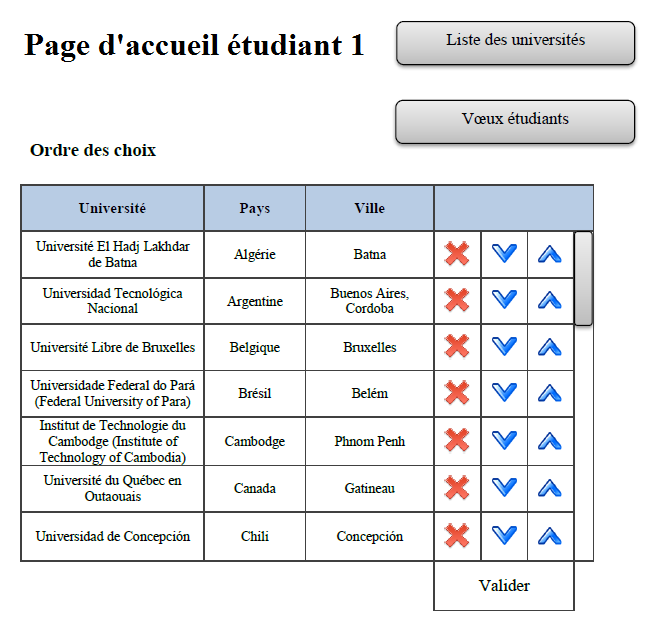
\includegraphics[scale=0.9]{Etudiant/HPS1.PNG}
	\caption{Page d'accueil pour les étudiants dans l'étape 1}
	\label{fig::hps1}
\end{figure}

La figure \ref{fig::hps1} des un aperçu de la page d'entrée du site pour les élèves.\\
Une fois identifiés via le CAS, ils sont dirigés vers une page qui est propre à chaque élève et qui se modifie selon ses choix.
Plusieurs élément sont présents sur cette page.

\bigbreak

Le premier est un tableau présentant les vœux de l'élèves sous forme d'une liste d'universités.

Chaque ligne du tableau correspond à une université, une ligne du tableau est composé de plusieurs champs qui donnent des informations sur l'université correspondante (comme le pays, la ville etc).

De plus chaque université est un lien vers une "Fiche université" (cf section \ref{sec::sheet_univ}) de cette université. Cette fiche donnera toutes les informations nécessaires sur cette université ainsi que les commentaires laissés par les autres élèves des années précédentes.

Le tableau de vœux possède des boutons pour effectuer les actions basiques comme ajouter, supprimer ou modifier ses vœux. Il y a également un bouton pour valider nos choix d'universités et informer les correspondants RI que cette liste est définitive. La réorganisation des vœux est néanmoins possible après validation de l'élève tant que le correspondant RI n'a pas fixé les vœux ;

\bigbreak

Un bouton redirigeant vers "Liste des Universités" (cf section \ref{sec::list_univ}) permet d'accéder à la liste de toutes les universités.

\bigbreak

Enfin, un bouton redirigeant vers "Vœux des Étudiants" (cf section \ref{sec::stud_wish}) permet d'accéder aux vœux des autres étudiants.
